%%
%% This is file `sample-sigconf-authordraft.tex',
%% generated with the docstrip utility.
%%
%% The original source files were:
%%
%% samples.dtx  (with options: `all,proceedings,bibtex,authordraft')
%% 
%% IMPORTANT NOTICE:
%% 
%% For the copyright see the source file.
%% 
%% Any modified versions of this file must be renamed
%% with new filenames distinct from sample-sigconf-authordraft.tex.
%% 
%% For distribution of the original source see the terms
%% for copying and modification in the file samples.dtx.
%% 
%% This generated file may be distributed as long as the
%% original source files, as listed above, are part of the
%% same distribution. (The sources need not necessarily be
%% in the same archive or directory.)
%%
%%
%% Commands for TeXCount
%TC:macro \cite [option:text,text]
%TC:macro \citep [option:text,text]
%TC:macro \citet [option:text,text]
%TC:envir table 0 1
%TC:envir table* 0 1
%TC:envir tabular [ignore] word
%TC:envir displaymath 0 word
%TC:envir math 0 word
%TC:envir comment 0 0
%%
%% The first command in your LaTeX source must be the \documentclass
%% command.
%%
%% For submission and review of your manuscript please change the
%% command to \documentclass[manuscript, screen, review]{acmart}.
%%
%% When submitting camera ready or to TAPS, please change the command
%% to \documentclass[sigconf]{acmart} or whichever template is required
%% for your publication.
%%
%%
% \documentclass[sigconf,authordraft]{acmart}
\documentclass[sigconf,review,anonymous,screen]{acmart}
% \documentclass[sigconf,review,screen]{acmart}
% \documentclass[sigconf]{acmart}

%%
%% \BibTeX command to typeset BibTeX logo in the docs
\AtBeginDocument{%
  \providecommand\BibTeX{{%
    Bib\TeX}}}

%% Rights management information.  This information is sent to you
%% when you complete the rights form.  These commands have SAMPLE
%% values in them; it is your responsibility as an author to replace
%% the commands and values with those provided to you when you
%% complete the rights form.
\setcopyright{acmlicensed}
\copyrightyear{2018}
\acmYear{2018}
\acmDOI{XXXXXXX.XXXXXXX}
%% These commands are for a PROCEEDINGS abstract or paper.
\acmConference[Conference acronym 'XX]{Make sure to enter the correct
  conference title from your rights confirmation email}{June 03--05,
  2018}{Woodstock, NY}
%%
%%  Uncomment \acmBooktitle if the title of the proceedings is different
%%  from ``Proceedings of ...''!
%%
%%\acmBooktitle{Woodstock '18: ACM Symposium on Neural Gaze Detection,
%%  June 03--05, 2018, Woodstock, NY}
\acmISBN{978-1-4503-XXXX-X/2018/06}


%%
%% Submission ID.
%% Use this when submitting an article to a sponsored event. You'll
%% receive a unique submission ID from the organizers
%% of the event, and this ID should be used as the parameter to this command.
%%\acmSubmissionID{123-A56-BU3}
\acmSubmissionID{3106}

\usepackage{multirow}
\usepackage{graphicx} % 用于 \resizebox
\usepackage{amssymb}  % 用于 \checkmark
%%
%% For managing citations, it is recommended to use bibliography
%% files in BibTeX format.
%%
%% You can then either use BibTeX with the ACM-Reference-Format style,
%% or BibLaTeX with the acmnumeric or acmauthoryear sytles, that include
%% support for advanced citation of software artefact from the
%% biblatex-software package, also separately available on CTAN.
%%
%% Look at the sample-*-biblatex.tex files for templates showcasing
%% the biblatex styles.
%%

%%
%% The majority of ACM publications use numbered citations and
%% references.  The command \citestyle{authoryear} switches to the
%% "author year" style.
%%
%% If you are preparing content for an event
%% sponsored by ACM SIGGRAPH, you must use the "author year" style of
%% citations and references.
%% Uncommenting
%% the next command will enable that style.
%%\citestyle{acmauthoryear}


%%
%% end of the preamble, start of the body of the document source.
\begin{document}

%%
%% The "title" command has an optional parameter,
%% allowing the author to define a "short title" to be used in page headers.
% \title{Beyond the Last Layer: Dynamic Scale-Aware Aggregation and Geometry-Guided Focus for Gaze Target Estimation}
\title{Gaze in the Crowd: Frustum-Aware Feature Aggregation for Robust Gaze Target Estimation}

%%
%% The "author" command and its associated commands are used to define
%% the authors and their affiliations.
%% Of note is the shared affiliation of the first two authors, and the
%% "authornote" and "authornotemark" commands
%% used to denote shared contribution to the research.
\author{Bin Fan}
\affiliation{%
  \institution{School of Computer Science and Engineering, University of Electronic Science and Technology of China}
  \city{Chengdu}
  \state{Sichuan}
  \country{China}
}
\email{202421080407@std.uestc.edu.cn}

\author{Tongjie Pan}
\affiliation{%
  \institution{School of Computer Science and Engineering, University of Electronic Science and Technology of China}
  \city{Chengdu}
  \state{Sichuan}
  \country{China}
}
\email{tongjiepan@foxmail.com}

\author{Huiyu Zhai}
\affiliation{%
  \institution{School of Computer Science and Engineering, University of Electronic Science and Technology of China}
  \city{Chengdu}
  \state{Sichuan}
  \country{China}
}
\email{huiyu.zhai@qq.com}

\author{Tao Zhou}
\affiliation{%
  \institution{School of Computer Science and Engineering, University of Electronic Science and Technology of China}
  \city{Chengdu}
  \state{Sichuan}
  \country{China}
}
\email{202521081139@std.uestc.edu.cn}

\author{Yalan Ye}
\affiliation{%
  \institution{School of Computer Science and Engineering, University of Electronic Science and Technology of China}
  \city{Chengdu}
  \state{Sichuan}
  \country{China}
}
\email{yalanye@uestc.edu.cn}



%%
%% By default, the full list of authors will be used in the page
%% headers. Often, this list is too long, and will overlap
%% other information printed in the page headers. This command allows
%% the author to define a more concise list
%% of authors' names for this purpose.
\renewcommand{\shortauthors}{Bin Fan, Tongjie Pan, Huiyu Zhai, Tao Zhou, Yalan Ye}

%%
%% The abstract is a short summary of the work to be presented in the
%% article.
% \begin{abstract}
%   Gaze target estimation aims to localize the final fixation point of a person within an image. Although recent methods have introduced Vision Foundation Models (VFMs), they typically exploit only the deepest features. This practice leads to a spatial-semantic dilemma. While deep representations are semantically rich, they lose the high-resolution geometric details essential for tracking subtle gaze directions. To break this information bottleneck, we propose a streamlined and highly efficient single-branch network. By unleashing the potential of multi-layer foundation features, our approach restores the geometric-semantic balance for gaze estimation. Specifically, we design two collaborative modules. First, the Scale-Aware Semantic Aggregation (SASA) module acts as a cognitive engine. It adaptively fuses shallow textures with deep semantics based on the global context, effectively addressing the feature granularity selection problem of "what to look at." Second, the Geometry-Guided Spatial Focus (GGSF) module introduces the physical prior of a viewing frustum. By constructing an explicit multiplicative mask via a relative coordinate field, GGSF acts like a spotlight. It actively highlights potential interaction regions in the line of sight while filtering out background noise, thereby solving the spatial focus problem of "where to look." Despite its minimalist architecture that relies on no additional modalities (e.g., depth or pose), 
%   % our method achieves SOTA performance on both the GazeFollow and VideoAttentionTarget datasets. 
%   we demonstrate SOTA performance across several gaze benchmark.
%   Code and pre-trained model will be released.
% \end{abstract}

\begin{abstract}
% Gaze target estimation is a challenging task due to severe contextual interference in complex, crowded scenes. Traditional multi-branch methods heavily rely on cumbersome architectures and auxiliary modalities, while recent single-branch models based on Vision Foundation Models (VFMs) blindly exploit only the deepest features. Especially in crowded environments, this over-reliance on deep representations causes VFMs to struggle with semantic confusion and lose the high-resolution geometric details essential for accurate gaze tracking. In response, we present GazeSpot, which unleashes multi-layer foundation features to restore the geometric-semantic balance, introducing two key contributions: First, we introduce a Geometry-Guided Spatial Focus (GGSF) module that leverages a physical frustum prior to construct an explicit multiplicative mask. Acting like a spotlight, GGSF proactively filters background noise and mitigates contextual interference to resolve the spatial focus problem. Second, we customize a Scale-Aware Semantic Aggregation (SASA) module to adaptively fuse shallow, occlusion-resistant textures with deep semantics based on the global context, effectively addressing the feature granularity selection. We further construct a specialized Crowd evaluation subset to facilitate robust benchmarking under severe social interference. Extensive experiments on general public benchmarks and the Crowd subset demonstrate that our proposed architecture achieves SOTA recognition performance. 
As a core capability for human intent inference, gaze target estimation remains challenging due to severe contextual interference in crowded scenes. Traditional multi-branch methods suffer from cumbersome architectures and heavy reliance on auxiliary modalities. Meanwhile, recent single-branch models based on Vision Foundation Models (VFMs) blindly exploit only the deepest features. Especially in crowded environments, this over-reliance on deep representations causes VFMs to struggle with semantic confusion and lose the high-resolution geometric details essential for accurate gaze tracking. To address this, we present GazeSpot, which unleashes multi-layer foundation features to restore the geometric-semantic balance via two key contributions: First, the Geometry-Guided Spatial Focus (GGSF) module leverages a physical frustum prior to generate an explicit multiplicative mask. Acting like a spotlight, GGSF proactively filters background noise and mitigates contextual interference to resolve spatial focus. Second, the Scale-Aware Semantic Aggregation (SASA) module adaptively fuses shallow, occlusion-resistant textures with deep semantics based on the global context, effectively addressing the feature granularity selection problem. We curate a specialized Crowd evaluation subset to facilitate robust benchmarking under severe social interference. Extensive experiments on general public benchmarks and the Crowd subset demonstrate that our method achieves state-of-the-art performance.
Code and pre-trained models will be released.
\end{abstract}

%%
%% The code below is generated by the tool at http://dl.acm.org/ccs.cfm.
%% Please copy and paste the code instead of the example below.
%%
\begin{CCSXML}
<ccs2012>
   <concept>
       <concept_id>10010147.10010178.10010224.10010225.10010227</concept_id>
       <concept_desc>Computing methodologies~Scene understanding</concept_desc>
       <concept_significance>500</concept_significance>
       </concept>
   <concept>
       <concept_id>10010147.10010257.10010293.10010294</concept_id>
       <concept_desc>Computing methodologies~Neural networks</concept_desc>
       <concept_significance>300</concept_significance>
       </concept>
   <concept>
       <concept_id>10003120.10003121</concept_id>
       <concept_desc>Human-centered computing~Human computer interaction (HCI)</concept_desc>
       <concept_significance>100</concept_significance>
       </concept>
 </ccs2012>
\end{CCSXML}

\ccsdesc[500]{Computing methodologies~Scene understanding}
\ccsdesc[300]{Computing methodologies~Neural networks}
\ccsdesc[100]{Human-centered computing~Human computer interaction (HCI)}

%%
%% Keywords. The author(s) should pick words that accurately describe
%% the work being presented. Separate the keywords with commas.
\keywords{Gaze Target Estimation, Vision Foundation Models, Spatial Attention, Multi-scale Feature Aggregation, Human Behavior Analysis}
%% A "teaser" image appears between the author and affiliation
%% information and the body of the document, and typically spans the
%% page.
% \begin{teaserfigure}
%   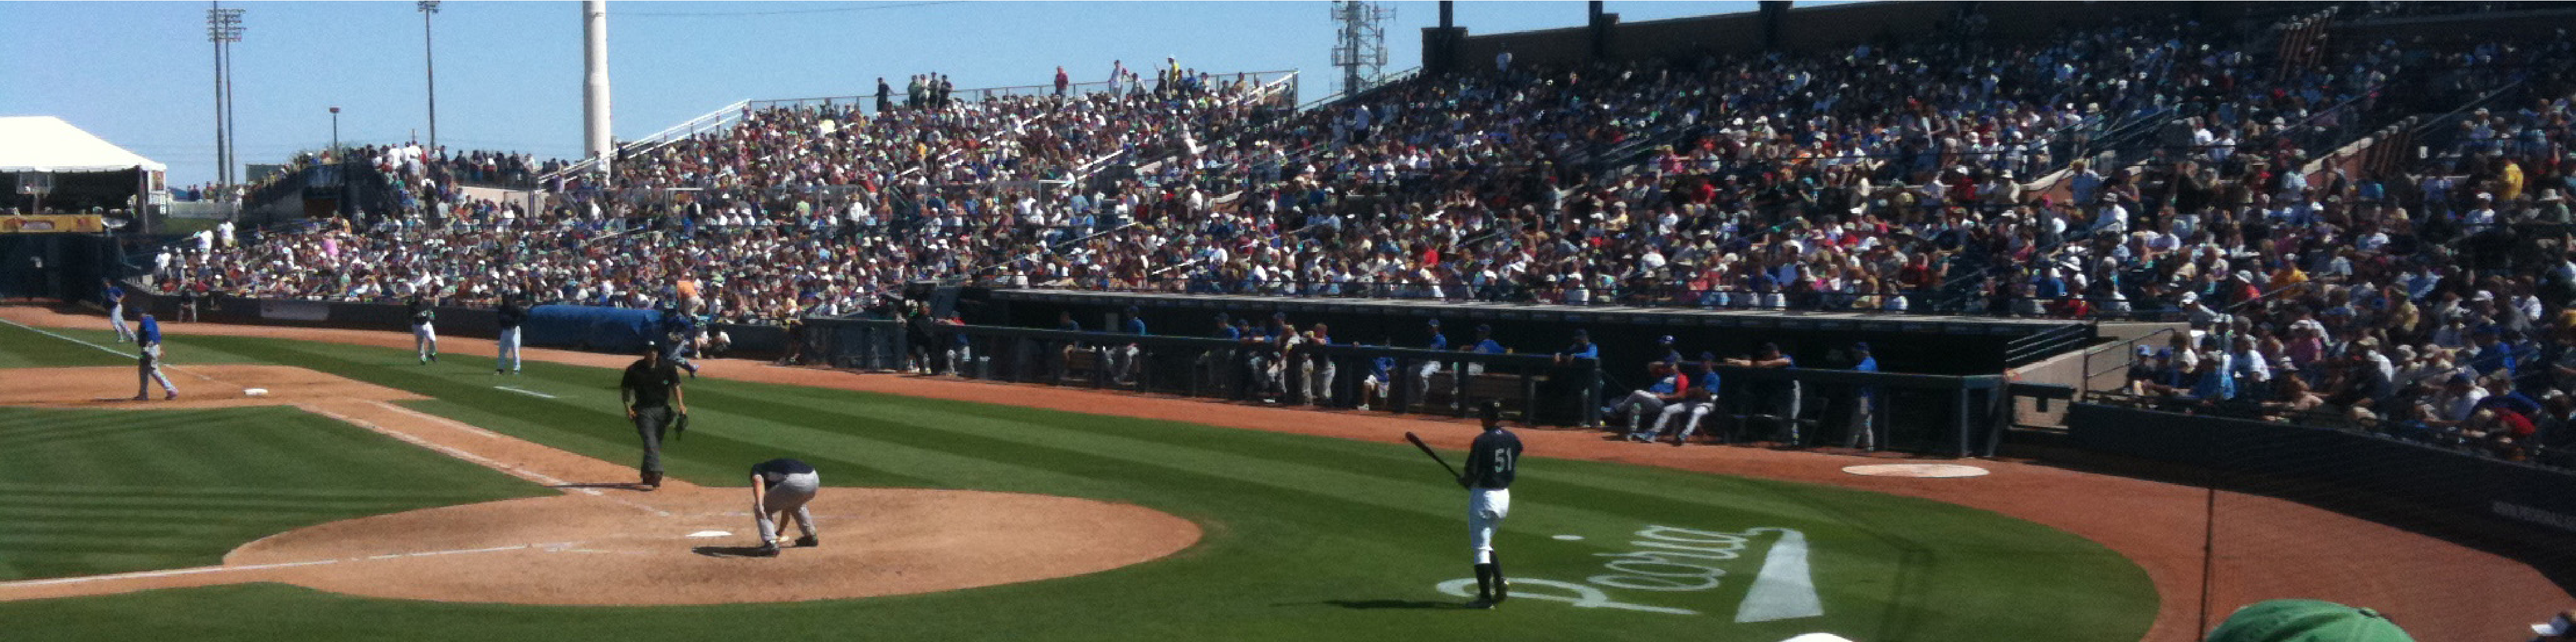
\includegraphics[width=\textwidth]{sampleteaser}
%   \caption{Seattle Mariners at Spring Training, 2010.}
%   \Description{Enjoying the baseball game from the third-base
%   seats. Ichiro Suzuki preparing to bat.}
%   \label{fig:teaser}
% \end{teaserfigure}

% \received{20 February 2007}
% \received[revised]{12 March 2009}
% \received[accepted]{5 June 2009}

%%
%% This command processes the author and affiliation and title
%% information and builds the first part of the formatted document.
\maketitle

\section{Introduction}
\label{sec:introduction}
\begin{figure}[t]
\vspace{15pt}
    % \begin{center}
    %    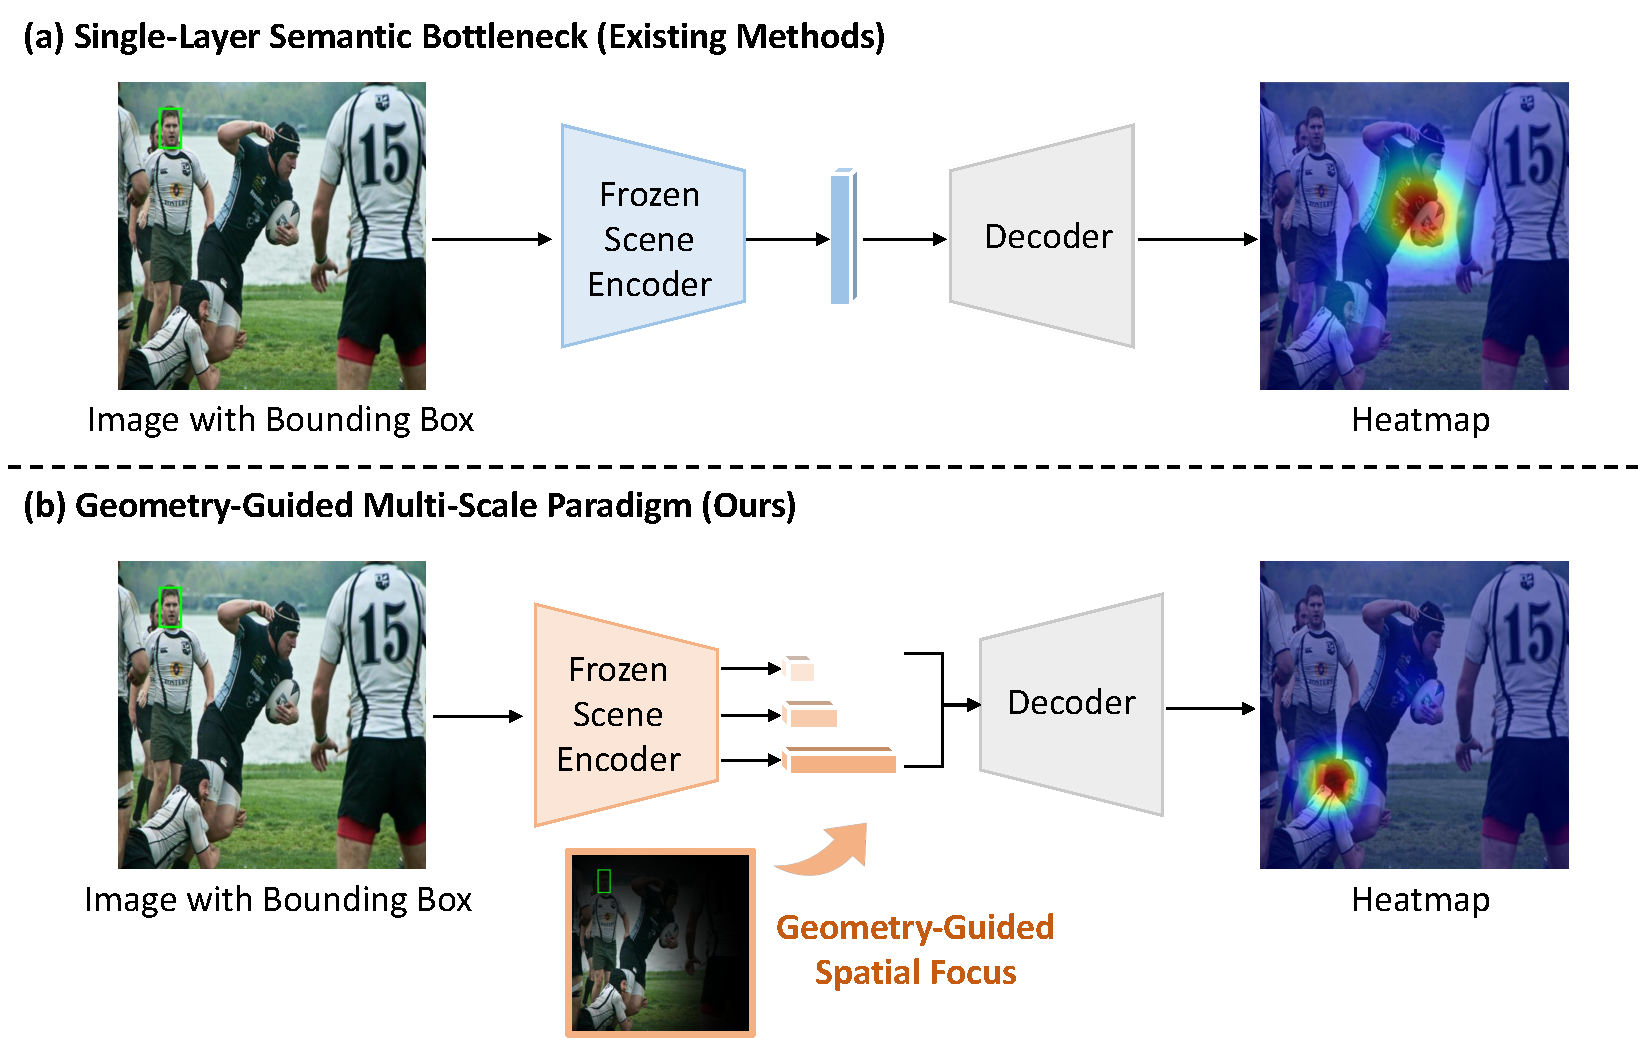
\includegraphics[width=1.0\linewidth]{Figure/teaser.pdf} 
    % \end{center}
    \centering
    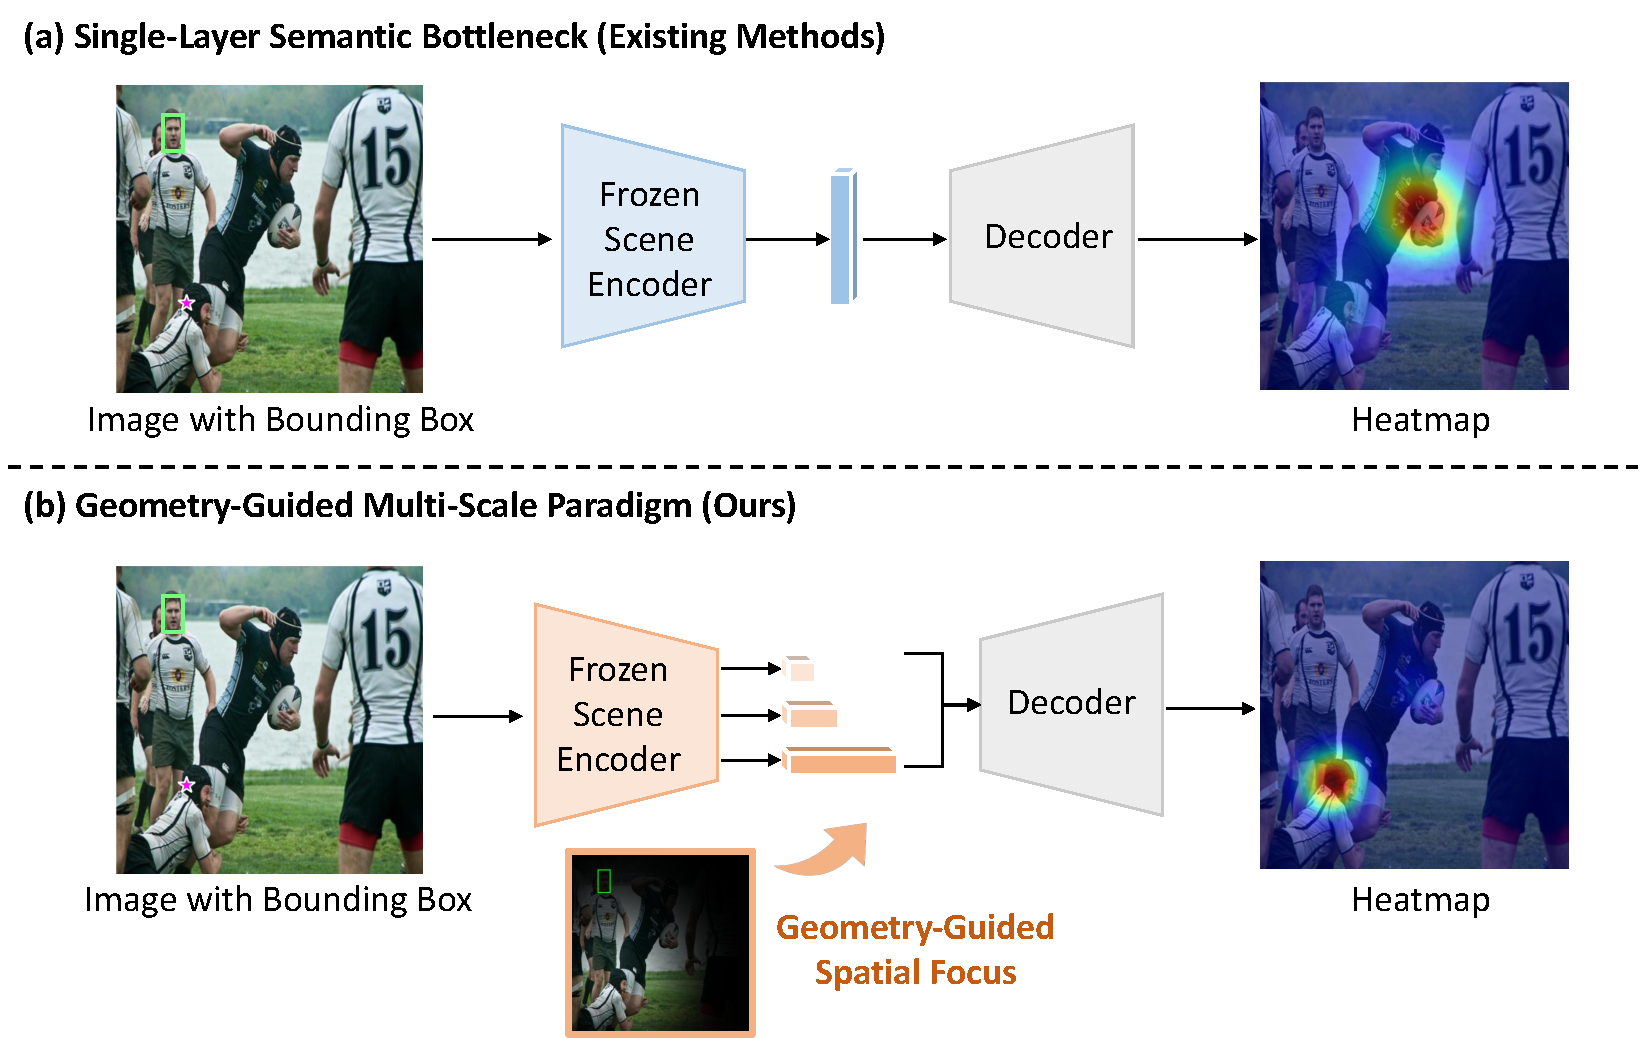
\includegraphics[width=\linewidth]{Figure/teaserV2.pdf} 
    \caption{Motivation comparison. Existing methods (top) exploit only the deepest foundation features, trapping themselves in the "spatial-semantic dilemma" with diffuse activations and lost geometric details. In contrast, our proposed GazeSpot (bottom) introduces a geometry-guided multi-scale mechanism, enabling a paradigm shift from "blind semantic reliance" to "adaptive geometric-semantic synergy."}
    \label{fig:teaser} 
% \vspace{-5pt}
\end{figure}
Gaze target estimation aims to infer the final fixation point of a person within an image~\cite{recasens2015they}. It serves as a core driving force for high-level semantic understanding in computer vision, such as human intent inference~\cite{fathi2012learning, huang2015using, lukander2017inferring, wei2018and}, human-computer interaction (HCI)~\cite{zander2010combining, noureddin2005non}, and social behavior analysis~\cite{emery2000eyes}. Given an image containing a person and their head bounding box, this task requires the model to not only precisely capture the 3D head pose~\cite{fischer2018rt,horanyi2023they} and subtle eyeball deflections~\cite{fang2021dual} but also possess a profound understanding of scene semantics~\cite{recasens2015they}. This is crucial for inferring the physical interaction between the gaze direction and scene objects.

Traditional gaze estimation methods heavily rely on complex multi-branch architectures~\cite{chong2020detecting,chen2021gaze,saran2018human,hu2022gaze,recasens2017following,wang2022gatector,zhao2020learning} (processing the head and scene independently) and auxiliary modalities like depth maps~\cite{bao2022escnet,horanyi2023they,tonini2022multimodal,guan2019enhanced}. Recently, inspired by the powerful generalization capabilities of Vision Foundation Models (VFMs), advanced methods like Gazelle~\cite{ryan2025gaze} have pioneered a minimalist single-branch paradigm. These approaches discard cumbersome feature fusion and auxiliary inputs, instead feeding the entire image into a frozen VFM and directly utilizing its final-layer features for unified scene representation and gaze decoding. However, a straightforward question arises: \textbf{\textit{Are these single-layer minimalist paradigms sufficiently robust in complex, real-world crowded scenes?}} To investigate this, we upgraded the backbone of a baseline model from DINOv2~\cite{oquab2023dinov2} to DINOv3~\cite{simeoni2025dinov3}, aiming to leverage its stronger semantic representation capabilities. Counterintuitively, the DINOv3-equipped model not only underperforms the DINOv2 baseline on the overall dataset, but the performance gap between them widens on the Crowd evaluation subset (detailed in \autoref{sec:experiments_45}).

Through in-depth analysis, we discovered that the blind reliance on the extremely deep features of large models traps them in a severe \textbf{spatial-semantic dilemma}. As illustrated by the Principal Component Analysis (PCA) visualization in \autoref{fig:v2VSv3}, during the layer-by-layer forward pass of VFMs, the model acquires high semantic homogeneity as the network depth increases and the receptive field expands drastically. Compared to DINOv2, the deepest features of DINOv3 exhibit severe \textbf{feature over-smoothing}~\cite{xie2023revealing} in crowded regions. Gaze estimation is not merely a semantic classification task; it is highly sensitive to geometric and physical properties~\cite{zhang2015appearance}. For instance, in highly dynamic multi-person interaction scenarios with occlusions (as shown in \autoref{fig:teaser}), when a person looks at a complex tackling action below, the model heavily depends on the fine spatial structures provided by shallow or middle-layer features to accurately track the gaze direction. However, the global receptive field of a single deep feature leads to severe \textbf{contextual interference} and \textbf{semantic confusion}. Consequently, the geometric features of the target person become entangled with adjacent salient distractors. This irreversible loss of high-resolution geometric details causes models utilizing only the last-layer features to easily have their attention hijacked~\cite{tafasca2024sharingan} in complex scenes, resulting in predictions that are diffuse, penetrate occlusions, or completely deviate from the target.

Motivated by this insight, to break the representation bottleneck imposed by a single deep layer, we propose an efficient single-branch gaze estimation framework named \textbf{GazeSpot}. This framework unleashes the potential of multi-layer foundation features for gaze inference without introducing significant computational overhead. Specifically, to address the aforementioned dilemma, we introduce two core designs to reconstruct the geometric-semantic balance.

First, deep networks are prone to losing relative spatial positions, leading to diffuse activation distributions. To counter this, we propose the \textbf{Geometry-Guided Spatial Focus (GGSF)} module. Abandoning the traditional practice of implicitly learning spatial positions, GGSF directly transforms the prior coordinates of the person's head into a physically meaningful relative distance field. Through a lightweight perceptron, GGSF maps this distance field into a spotlight-like frustum mask(Spotlight Mask). During the early stages of feature fusion, GGSF employs a multiplicative gating mechanism to act as a physical shield. It proactively filters out background activations outside the gaze cone, fundamentally cutting off contextual interference and resolving the "where to look" spatial focus problem.

Second, to overcome the limitations of feature over-smoothing in single-layer representations, we design the \textbf{Scale-Aware Semantic Aggregation (SASA)} mechanism. SASA performs global context perception across multi-layer features (shallow, middle, and deep) to dynamically compute attention weights for features at each scale. This mechanism acts as the model's cognitive engine, enabling it to adaptively route features based on image content. In crowded scenes, it intelligently invokes shallow textures to provide occlusion-resistant sharp edges, achieving optimal recombination with deep semantics. This effectively solves the feature granularity selection problem of "what to look at."

This dual design endows GazeSpot with both multi-scale semantic capacity and strict spatial geometric constraints. Furthermore, to accurately evaluate the model's anti-interference capability in complex social scenarios, we specifically curated a \textbf{Crowd evaluation subset}. Under a minimalist setup with no auxiliary modality inputs, our method not only demonstrates excellent performance on general benchmarks but also proves its robustness in highly challenging crowded scenes.

The core contributions of this paper are summarized as follows:
\begin{itemize}
    \item \textbf{New Perspective.} We deeply reveal the "spatial-semantic dilemma" and contextual interference faced by single-branch VFM models in crowded scenes. We demonstrate the necessity of introducing multi-layer feature adaptive routing to restore geometric perception capabilities.
    \item \textbf{New Module.} We propose the Geometry-Guided Spatial Focus module. By constructing an explicit relative distance field and frustum isolation, it effectively cuts off the interference of background noise, significantly enhancing the model's spatial focus capability and interpretability.
    \item \textbf{New Mechanism.} We propose the Scale-Aware Semantic Aggregation mechanism, endowing the model with cross-scale feature routing capabilities to dynamically allocate shallow occlusion-resistant textures and deep global semantics based on the global context.
    \item \textbf{New State-of-the-Art.} We curated a Crowd evaluation subset specifically targeting multi-person interference. GazeSpot not only achieves new SOTA performance on the general GazeFollow and VideoAttentionTarget datasets but also exhibits remarkable robustness advantages on the Crowd subset.
\end{itemize}
\begin{figure}[t]
% \vspace{15pt}
    \centering
    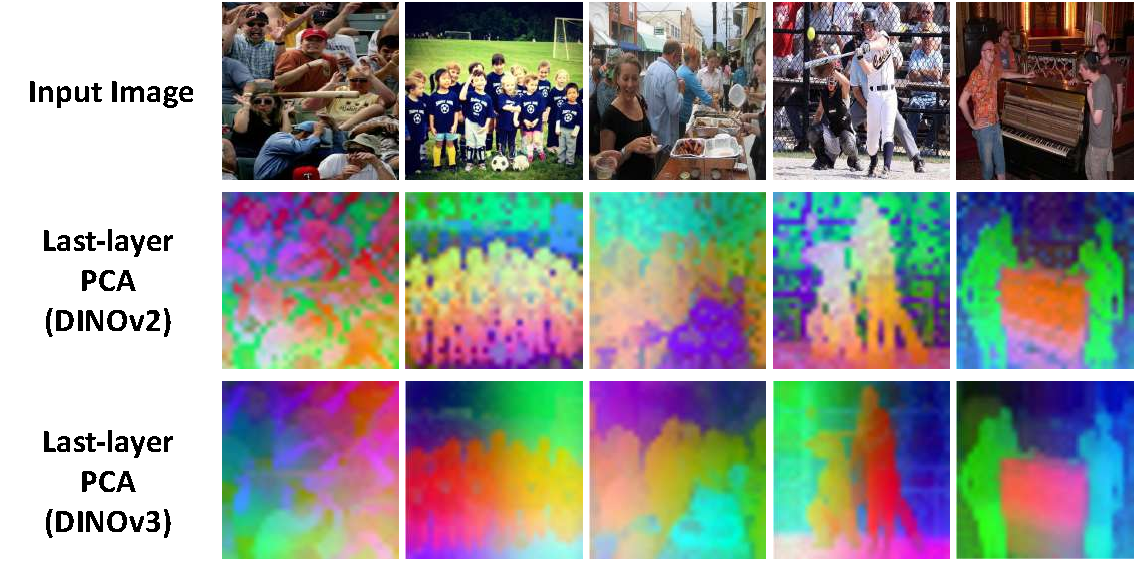
\includegraphics[width=\linewidth]{Figure/dinov2VSdinov3_compressed.pdf} 
    \caption{PCA visualization of the last-layer features from DINOv2 and DINOv3 in crowded scenes. While DINOv3 possesses stronger global semantic representations, it exhibits severe feature over-smoothing compared to DINOv2. This semantic homogeneity blurs the geometric boundaries between distinct individuals, causing severe contextual interference and the spatial-semantic dilemma in gaze estimation.}
    \label{fig:v2VSv3} 
% \vspace{-5pt}
\end{figure}

\section{Related Work}
\label{sec:related}

\subsection{Gaze Target Estimation Paradigms}
\label{subsec:paradigm}
Early approaches to gaze target estimation established multi-branch architectures as the dominant paradigm. Recasens et al.~\cite{recasens2015they} pioneered independent encoders for head crops and scene images, while Chong et al.~\cite{chong2020detecting} extended this framework to video sequences, introducing temporal modeling for dynamic scenes. Subsequent works incorporated multi-modal cues, with Fang et al.~\cite{fang2021dual} and Gupta et al.~\cite{gupta2022modular} integrating depth and pose estimation to enhance spatial reasoning, while Tonini et al.~\cite{tonini2023object} incorporated explicit object detection branches.  However, these methods rely on complex cross-branch fusion and auxiliary models, resulting in parameter-heavy architectures sensitive to modality noise. Recently, Ryan et al.~\cite{ryan2025gaze} and Song et al.~\cite{song2024vitgaze} shifted toward single-branch foundation model paradigms using frozen DINOv2 encoders~\cite{oquab2023dinov2}, significantly simplifying architectures while achieving competitive performance. Nevertheless, these approaches typically depend on single-layer deep representations, which may limit fine-grained spatial reasoning in complex scenes.

\subsection{Representation Learning for Dense Prediction}
\label{subsec:representation}

While Vision Foundation Models such as DINOv2 provide powerful semantic representations, deep features exhibit inherent limitations in dense prediction tasks. Caron et al.~\cite{caron2021emerging} and Sim\'eoni et al.~\cite{simeoni2021localizing} observed that self-supervised transformers tend toward feature over-smoothing, progressively losing fine-grained spatial details as the receptive field expands. For gaze estimation specifically, Kellnhofer et al.~\cite{kellnhofer2019gaze360} emphasized that accurate localization relies on high-resolution geometric cues such as subtle head pose variations, while Chong et al.~\cite{chong2020detecting} noted that distinguishing targets among spatially proximal distractors requires preserving fine spatial structures. These observations suggest that aggregating hierarchical representationss~\cite{lin2017feature} is necessary to balance semantic abstraction and geometric precision, rendering single-layer representations insufficient for crowded scenarios.

\subsection{Spatial Modeling and Attention Constraints}
\label{subsec:spatial}

Contemporary gaze estimation systems predominantly employ attention mechanisms for spatial modeling. Dosovitskiy et al.~\cite{dosovitskiy2020image} demonstrated that Transformers capture long-range dependencies through self-attention, yet such mechanisms provide only soft constraints on spatial relationships. Tafasca et al.~\cite{tafasca2024sharingan} observed that in crowded scenes, the indiscriminate global receptive field of deep attention layers introduces contextual interference, causing feature entanglement between adjacent individuals. To mitigate this, Kellnhofer et al.~\cite{kellnhofer2019gaze360} proposed geometric gaze fields, while Dai et al.~\cite{dai2025gazetarget360} explored multi-scale fusion for omnidirectional gaze estimation. However, existing approaches either lack explicit geometric isolation or employ rigid geometric assumptions without scene adaptability. Consequently, implicit attention alone remains insufficient for reliable gaze localization in complex, cluttered environments.

\section{Method}
\begin{figure*}[t]
    \begin{center}
        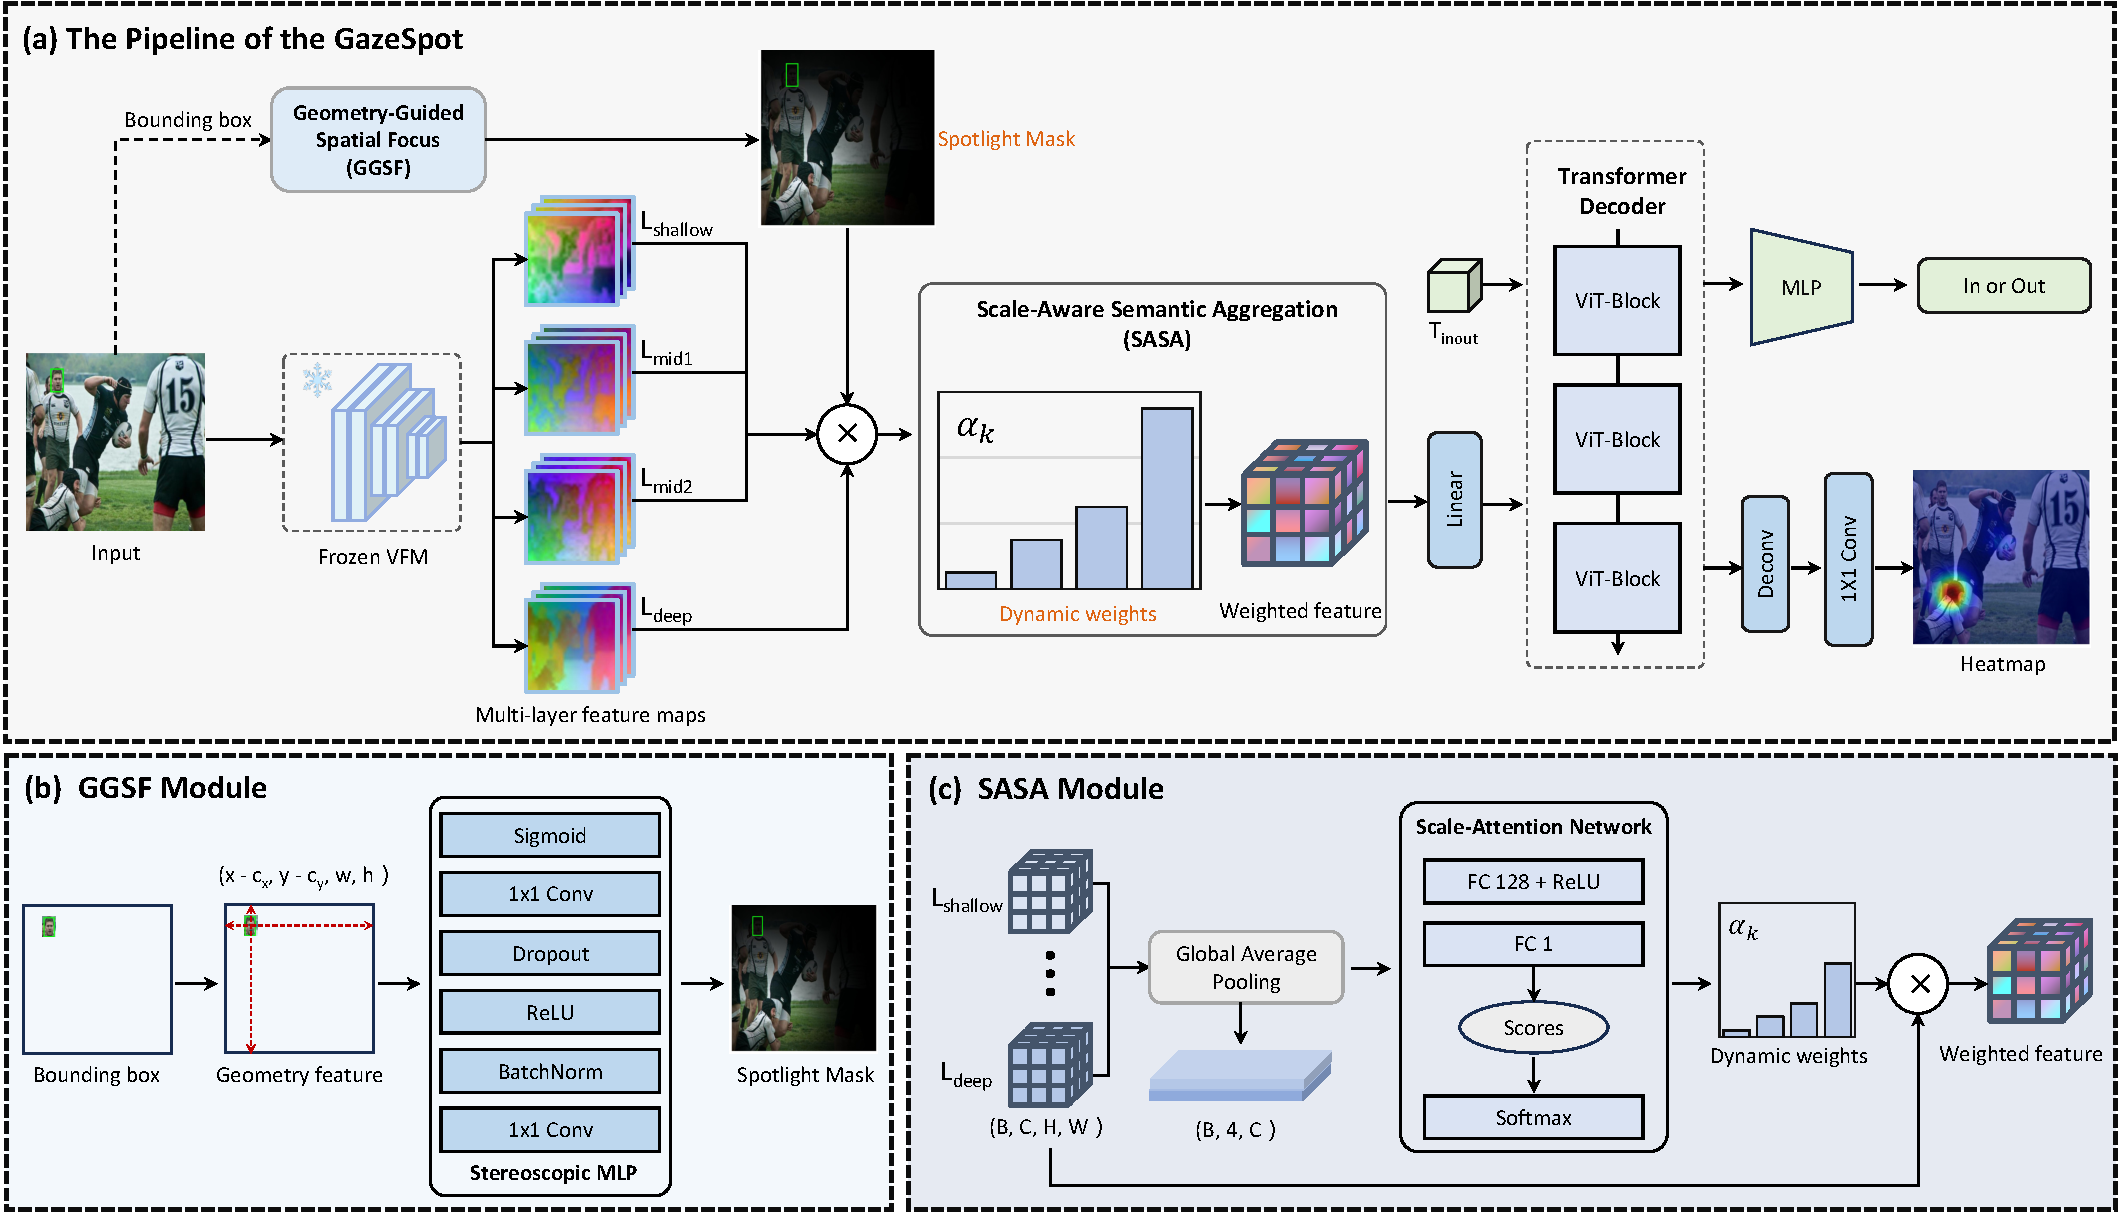
\includegraphics[width=0.95\textwidth]{Figure/pipelineV2.pdf}
    \end{center}
    \caption{Illustration of GazeSpot. (a) illustrates the overall pipeline. The input image is fed into a frozen VFM to extract multi-layer foundation features. These features first interact with the explicit frustum prior through the Geometry-Guided Spatial Focus (GGSF) module to proactively filter out background noise. Then, the Scale-Aware Semantic Aggregation (SASA) module dynamically allocates attention weights to adaptively fuse the spatially-filtered features across different scales. Finally, the fused representations are decoded by a lightweight Transformer to predict the gaze heatmap and out-of-frame probability. (b) shows the details of the GGSF module, which generates a Spotlight Mask via a stereoscopic MLP based on a relative coordinate field. (c) shows the details of the SASA module, which acts as a cognitive engine for cross-scale feature routing.}
    \label{fig:pipeline}
\end{figure*}
\subsection{Overall Architecture}

Given an input image $I \in \mathbb{R}^{3 \times H_I \times W_I}$ containing a target person and their corresponding head bounding box $\mathbf{b} = [x_{min}, y_{min}, x_{max}, y_{max}]$, our objective is to predict a probability heatmap $\mathbf{M} \in [0, 1]^{H_o \times W_o}$, where the position of the maximum value represents the final fixation point of the person's gaze.

As illustrated in \autoref{fig:pipeline}, we propose \textbf{GazeSpot}, a highly efficient single-branch network designed to break the representation bottleneck imposed by single-layer features of foundation models. The overall architecture consists of three core stages:

\textbf{(1) Foundation Feature Extraction:} We employ a pre-trained vision foundation model (e.g., DINOv3) as a frozen feature encoder. Unlike previous methods that exploit only the deepest features, we explicitly extract $K$ intermediate features uniformly distributed across different depths of the network to construct a multi-scale feature hierarchy $\mathcal{F} = \{\mathbf{F}_k\}_{k=1}^K$ that encompasses both fine-grained geometry and global semantics.

\textbf{(2) Geometric and Semantic Routing:} This is our core contribution. First, the \textbf{Geometry-Guided Spatial Focus (GGSF)} module leverages the physical coordinates of the head to generate an explicit viewing frustum mask, performing spatial filtering on the multi-layer features $\mathcal{F}$ to proactively filter out irrelevant backgrounds. Subsequently, the \textbf{Scale-Aware Semantic Aggregation (SASA)} module acts as a cognitive engine. It adaptively assigns attention weights to features of different scales based on the global context and fuses them along the channel dimension into a highly condensed scene representation.

\textbf{(3) Gaze Decoding and Out-of-Frame Prediction:} The fused representation, combined with positional encodings and the head position prior, is fed into a lightweight Transformer decoder alongside a dedicated state token. The network ultimately outputs a high-resolution gaze heatmap and the classification probability of whether the target is out-of-frame in parallel.

\subsection{Geometry-Guided Spatial Focus (GGSF)}

Deep vision networks often lose relative spatial position information during the encoding process, leading to a diffuse activation distribution when predicting gaze directions. To address this pain point, we abandon the conventional practice of implicitly learning spatial positions by stacking convolutions. Instead, we propose to introduce an explicit geometric prior via the GGSF module.

The core intuition behind GGSF is to construct a ``spotlight-like'' attention mechanism for the network. Specifically, for any spatial location $\mathbf{p} = (x, y)$ on the feature map, we first calculate its relative coordinates with respect to the person's head center $\mathbf{c} = (c_x, c_y)$. To endow this coordinate field with scale-aware capability, we further concatenate the absolute physical dimensions of the head (width $w$ and height $h$). Consequently, we construct a 4-channel geometric tensor $\mathbf{G} \in \mathbb{R}^{4 \times H \times W}$ as follows:
\begin{equation}
\label{eq:geometric_tensor}
    \begin{aligned}
    \mathbf{G}(\mathbf{p}) = \left[ x - c_x, y - c_y, w, h \right]
    \end{aligned}
\end{equation}

Subsequently, we feed $\mathbf{G}$ into a lightweight Multi-Layer Perceptron (MLP), consisting of two $1 \times 1$ convolutional layers, BatchNorm, and ReLU activations, to generate a spatial gating mask $\mathbf{M}_{geo} \in \mathbb{R}^{1 \times H \times W}$ with values ranging in $[0, 1]$:
\begin{equation}
\label{eq:spatial_mask}
    \begin{aligned}
    \mathbf{M}_{geo} = \sigma\left( \text{MLP}(\mathbf{G}) \right)
    \end{aligned}
\end{equation}
where $\sigma$ denotes the Sigmoid activation function. Notably, we scale up the bias initialization of the last MLP layer (e.g., set to $2.0$) to ensure that the mask values are close to $1$ during the early stages of training, thereby preserving the stability of the pre-trained VFM features.

Finally, by employing a multiplicative gating mechanism, the spatial mask $\mathbf{M}_{geo}$ is applied element-wise to the feature maps $\mathbf{F}_k$ at each scale, as described in \autoref{eq:gated_feature}, thereby proactively erasing irrelevant background noise outside the ``gaze cone'' during the early stages of feature fusion.
\begin{equation}
\label{eq:gated_feature}
    \begin{aligned}
    \mathbf{F}_k^{geo} = \mathbf{F}_k \otimes \mathbf{M}_{geo}, \quad \forall k \in \{1, \dots, K\}
    \end{aligned}
\end{equation}
This explicit spatial constraint significantly reduces the search space for subsequent semantic optimization.

\subsection{Scale-Aware Semantic Aggregation (SASA)}

After the spatial filtering by GGSF, the model must determine which layer of features to rely on more heavily for the current gaze scenario. For instance, in a densely crowded scene, distinguishing the specific target person's gaze direction from adjacent individuals heavily relies on the sharp geometric boundaries provided by shallow layers, whereas understanding the overarching social interaction or the salient distal object being looked at demands the global semantic context from deep layers. To this end, we propose the SASA module, endowing the model with cross-scale dynamic routing capabilities.

Given the geometry-gated multi-layer feature set $\{\mathbf{F}_k^{geo}\}_{k=1}^K$, where $\mathbf{F}_k^{geo} \in \mathbb{R}^{C \times H \times W}$, we first extract a global semantic descriptor $\mathbf{v}_k \in \mathbb{R}^C$ for each layer via Global Average Pooling (GAP):
\begin{equation}
\label{eq:gap}
    \begin{aligned}
    \mathbf{v}_k = \frac{1}{H \times W} \sum_{i=1}^H \sum_{j=1}^W \mathbf{F}_k^{geo}(i, j)
    \end{aligned}
\end{equation}

Next, we utilize a shared scale-attention network to evaluate the relative importance of each descriptor for the current scene, and normalize them across the scale dimension via a Softmax function to obtain dynamic weights $\alpha_k$:
\begin{equation}
\label{eq:dynamic_weights}
    \begin{aligned}
    \alpha_k = \frac{\exp(\mathbf{W}_2 \delta(\mathbf{W}_1 \mathbf{v}_k))}{\sum_{j=1}^K \exp(\mathbf{W}_2 \delta(\mathbf{W}_1 \mathbf{v}_j))}
    \end{aligned}
\end{equation}
where $\mathbf{W}_1$ and $\mathbf{W}_2$ represent the weights of fully connected layers, and $\delta$ denotes the ReLU activation function.

Upon obtaining the weights, SASA adaptively weights the features and concatenates them along the channel dimension. A $1 \times 1$ convolution is then applied to reduce the dimension to a unified hidden dimension $D$ ($D=256$ in this paper), yielding the final aggregated feature $\mathbf{X} \in \mathbb{R}^{D \times H \times W}$:
\begin{equation}
\label{eq:aggregated_feature}
    \begin{aligned}
    \mathbf{X} = \text{Conv}_{1 \times 1}\left( \text{Concat}_{k=1}^K (\alpha_k \cdot \mathbf{F}_k^{geo}) \right)
    \end{aligned}
\end{equation}

The ingenuity of SASA lies in liberating the network from the representation bottleneck of any single depth. Instead, it transforms the network into a flexible system capable of dynamically allocating the ``geometric-semantic'' synergy based on the image content.

\subsection{Gaze Decoding and Out-of-Frame Prediction}

In real-world video interaction scenarios (e.g., the VideoAttentionTarget dataset), a person's gaze target often lies out-of-frame. To construct a comprehensive gaze estimation system, our decoder must not only predict in-frame gaze heatmaps but also possess the binary classification capability to determine whether the target is within the frame.

Given the 2D feature $\mathbf{X}$ fused by SASA, we first flatten its spatial dimensions and transpose it into a 1D feature sequence $\mathbf{S} \in \mathbb{R}^{(HW) \times D}$. To preserve spatial position information and the person identity prior, we perform an element-wise addition of the sequence with a learnable 2D positional encoding $\mathbf{E}_{pos}$~\cite{dosovitskiy2020image} and a head map embedding $\mathbf{E}_{head}$:
\begin{equation}
\label{eq:sequence_addition}
    \begin{aligned}
    \mathbf{S}' = \mathbf{S} + \mathbf{E}_{pos} + \mathbf{E}_{head}
    \end{aligned}
\end{equation}
where $\mathbf{E}_{head}$ is obtained by mapping the person's original bounding box region into a mask and multiplying it by a learnable head token. This is designed to explicitly guide the model to focus on the specific person currently under test.

To enable out-of-frame gaze prediction, we introduce a dedicated learnable token $\mathbf{T}_{inout} \in \mathbb{R}^{1 \times D}$, concatenated at the forefront of the sequence:
\begin{equation}
\label{eq:sequence_concat}
    \begin{aligned}
    \mathbf{S}_{input} = [\mathbf{T}_{inout}, \mathbf{S}']
    \end{aligned}
\end{equation}

Subsequently, the complete sequence $\mathbf{S}_{input}$ is fed into an encoder consisting of $L$ ($L=3$ in this paper) standard Transformer blocks~\cite{vaswani2017attention}. Leveraging the self-attention mechanism, the model can perform deep, cross-domain information interaction between head features and scene context within a global receptive field.

The output sequence of the Transformer is denoted as $[\hat{\mathbf{T}}_{inout}, \hat{\mathbf{S}}]$. We separate it to perform two parallel tasks:

\textbf{(1) Out-of-Frame Prediction:} The initial token $\hat{\mathbf{T}}_{inout}$ is fed into a classification head composed of an MLP to predict the probability $\hat{p}_{inout}$ that the fixation point is located within the frame:
\begin{equation}
\label{eq:out_of_frame_prob}
    \begin{aligned}
    \hat{p}_{inout} = \sigma(\text{MLP}(\hat{\mathbf{T}}_{inout}))
    \end{aligned}
\end{equation}

\textbf{(2) Gaze Heatmap Generation:} The remaining sequence $\hat{\mathbf{S}}$ is reshaped back into a 2D feature map and fed into a heatmap decoding head (comprising deconvolutional upsampling and a $1 \times 1$ convolution). This ultimately outputs a high-resolution gaze probability heatmap $\hat{\mathbf{M}} \in [0, 1]^{H_o \times W_o}$:
\begin{equation}
\label{eq:heatmap_generation}
    \begin{aligned}
    \hat{\mathbf{M}} = \sigma(\text{Deconv}(\text{Reshape}(\hat{\mathbf{S}})))
    \end{aligned}
\end{equation}

\subsection{Optimization Objective}

During the end-to-end training process, we unify the heatmap prediction and out-of-frame gaze prediction into pixel-level and image-level Binary Cross-Entropy (BCE) optimization problems.

For in-frame gaze heatmap prediction, since the fixation point is typically modeled as a Gaussian distributed region, we employ the BCE Loss to pixel-wisely constrain the difference between the predicted heatmap $\hat{\mathbf{M}}$ and the ground-truth Gaussian heatmap $\mathbf{M}_{gt}$:
% \begin{equation}
% \label{eq:loss_heat}
%     % \begin{aligned}
%     \mathcal{L}_{heat} = -\frac{1}{H_o W_o} \sum_{i,j} \left[ \mathbf{M}_{gt}^{i,j} \log \hat{\mathbf{M}}^{i,j} + (1 - \mathbf{M}_{gt}^{i,j}) \log (1 - \hat{\mathbf{M}}^{i,j}) \right]
%     % \end{aligned}
% \end{equation}
\begin{equation}
\label{eq:loss_heat}
    \mathcal{L}_{heat} = -\frac{1}{H_o W_o} \sum_{i,j} \bigl[ \mathbf{M}_{gt}^{i,j} \log \hat{\mathbf{M}}^{i,j} + (1 - \mathbf{M}_{gt}^{i,j}) \log (1 - \hat{\mathbf{M}}^{i,j}) \bigr]
\end{equation}

For out-of-frame gaze classification, we similarly use the BCE Loss to constrain the predicted probability $\hat{p}_{inout}$ against the ground-truth binary label $p_{gt} \in \{0, 1\}$ ($1$ indicates in-frame, $0$ indicates out-of-frame):
\begin{equation}
\label{eq:loss_inout}
    \begin{aligned}
    \mathcal{L}_{inout} = -\left[ p_{gt} \log \hat{p}_{inout} + (1 - p_{gt}) \log (1 - \hat{p}_{inout}) \right]
    \end{aligned}
\end{equation}

The final overall optimization objective function $\mathcal{L}_{total}$ is the weighted sum of the two, as described in \autoref{eq:loss_total}, where $\lambda$ is a hyperparameter balancing the two tasks.
\begin{equation}
\label{eq:loss_total}
    \begin{aligned}
    \mathcal{L}_{total} = \mathcal{L}_{heat} + \lambda \mathcal{L}_{inout}
    \end{aligned}
\end{equation}
Specifically, on datasets containing only in-frame gaze (e.g., GazeFollow), $\lambda$ is set to $0$; whereas on datasets containing out-of-frame gaze (e.g., VideoAttentionTarget), this term is activated.

\section{Experiments}
\label{sec:experiments}

\subsection{Datasets and Evaluation Metrics}
To comprehensively evaluate the performance and robustness of GazeSpot, we conduct extensive experiments on two highly challenging and authoritative large-scale public datasets, and specifically construct an evaluation subset tailored for crowded scenes.

\begin{table}[h]
  \centering
  \caption{Sample distribution of the Crowd Subset across different density levels.}
  \label{tab:crowd_distribution}
  \begin{tabular}{lc}
    \toprule
    \textbf{Scene Density (BBoxes)} & \textbf{Number of Samples (Frames)} \\
    \midrule
    $<3$ (Sparse) & 7,945 \\
    $3$ (Moderate) & 3,015 \\
    $4$ (Crowded) & 1,628 \\
    $>4$ (Extremely Crowded) & 539 \\
    \bottomrule
  \end{tabular}
\end{table}
\textbf{GazeFollow}~\cite{recasens2015they}: This dataset is the most widely used benchmark in the field of gaze target estimation, comprising a massive number of static images in real-world scenarios. Since the same person in an image may correspond to different fixation points annotated by multiple annotators, this dataset primarily evaluates the model's spatial inference capabilities in complex scenes.

% [Placeholder for Table 2: Comparison with State-of-the-Art methods on GazeFollow and VideoAttentionTarget datasets]
\begin{table*}[t]
  \centering
  \caption{Comparison with State-of-the-Art methods on GazeFollow and VideoAttentionTarget datasets. The best results are highlighted in bold.}
  \label{tab:sota_comparison}
  \begin{tabular}{llccccccccc}
    \toprule
    \multirow{2}{*}{\textbf{Category}} & \multirow{2}{*}{\textbf{Methods}} & \multirow{2}{*}{\textbf{Venue}} & \multirow{2}{*}{\textbf{Params}} & \multicolumn{3}{c}{\textbf{GazeFollow}} & \multicolumn{3}{c}{\textbf{VideoAttentionTarget}} \\
    \cmidrule(lr){5-7} \cmidrule(lr){8-10}
    & & & & \textbf{AUC} $\uparrow$ & \textbf{Avg $L_2$} $\downarrow$ & \textbf{Min $L_2$} $\downarrow$ & \textbf{AUC} $\uparrow$ & \textbf{$L_2$} $\downarrow$ & \textbf{In/Out AP} $\uparrow$ \\
    \midrule
    \multirow{9}{*}{\shortstack[l]{Multi-branch / \\ Multi-modal}} 
    & Chong et al.~\cite{chong2018connecting} & ECCV 2018 & 51M & 0.896 & 0.187 & 0.112 & 0.833 & 0.171 & 0.712 \\
    & Lian et al.~\cite{lian2018believe} & ACCV 2018 & 55M & 0.906 & 0.145 & 0.081 & 0.837 & 0.165 & - \\
    & Chong et al.~\cite{chong2020detecting}& CVPR 2020 & 61M & 0.921 & 0.137 & 0.077 & 0.860 & 0.134 & 0.853 \\
    & Fang et al.~\cite{fang2021dual} & CVPR 2021 & 68M  & 0.922 & 0.124 & 0.067 & 0.905 & 0.108 & 0.896 \\
    & Bao et al.~\cite{bao2022escnet} & CVPR 2022  & 29M & 0.928 & 0.122 & - & 0.885 & 0.120 & 0.869 \\
    & Jin et al.~\cite{jin2022depth} & EAAI 2022 & 52M  & 0.920 & 0.118 & 0.063 & 0.900 & 0.104 & 0.895 \\
    & Miao et al.~\cite{miao2023patch} & WACV 2023 & 61M  & 0.934 & 0.123 & 0.065 & 0.917 & 0.109 & \underline{0.908} \\
    & Tafasca et al.~\cite{tafasca2023childplay} & ICCV 2023 & 25M  & 0.939 & 0.122 & 0.062 & 0.914 & 0.109 & 0.834 \\
    & Tafasca et al.~\cite{tafasca2024sharingan} & CVPR 2024 & 105M  & 0.944 & 0.113 & 0.057 & - & 0.107 & 0.891 \\
    \midrule
    \multirow{4}{*}{\shortstack[l]{VFM-based \\ Single-branch}} 
    & ViTGaze~\cite{song2024vitgaze}  & VI 2024 & 22M  & 0.949 & 0.105 & 0.047 & \underline{0.938} & \underline{0.102} & 0.905 \\
    & GT360~\cite{dai2025gazetarget360}  & IROS 2025 & 1.9M & 0.957 & 0.101 & - & 0.934 & 0.103 & 0.887 \\
    & Gaze-LLE(ViT-B)~\cite{ryan2025gaze}  & CVPR 2025 & 2.8M & 0.956 & 0.104 & 0.045 & 0.933 & 0.107 & 0.897 \\
    & Gaze-LLE(ViT-L)~\cite{ryan2025gaze}  & CVPR 2025  & 2.9M & \underline{0.958} & \underline{0.099} & \underline{0.041} & 0.937 & 0.103 & 0.903 \\
    \midrule
    \multirow{2}{*}{\textbf{Ours}} 
    & \textbf{GazeSpot (ViT-B)}  & \textbf{-}  & 3.5M & \underline{0.958} & 0.101 & 0.043 & \textbf{0.940} & \textbf{0.099} & 0.887 \\
    & \textbf{GazeSpot (ViT-L)} & \textbf{-} & 3.8M & \textbf{0.961} & \textbf{0.093} & \textbf{0.038} & \textbf{0.944} & \textbf{0.092} & \textbf{0.912} \\
    \bottomrule
  \end{tabular}
\end{table*}
\textbf{VideoAttentionTarget (VAT)}~\cite{chong2020detecting}: This is a large-scale, highly dynamic video dataset. Unlike GazeFollow, VAT not only contains complex social interactions but also introduces ``out-of-frame'' gaze annotations, requiring the model to possess the binary classification capability to determine whether the target falls outside the image boundaries.

\textbf{Crowd Subset}: To precisely quantify the model's robustness against contextual interference, we conduct a fine-grained reconstruction of the test set from the VAT dataset. Specifically, we strictly categorize the test samples into four density levels based on the number of ground truth head bounding boxes in each frame: $<3$ (Sparse), $3$ (Moderate), $4$ (Crowded), and $>4$ (Extremely Crowded). This rigorous quantitative division allows us to clearly track the performance degradation trajectory of models as the number of distractors increases. The specific frame distribution across different density levels is detailed in \autoref{tab:crowd_distribution}.

\textbf{Evaluation Metrics}: Regarding evaluation metrics, we strictly adhere to the standard protocols of this field. For in-frame gaze, we employ AUC (Area Under Curve) by treating the heatmap as classification confidences to evaluate overall prediction accuracy. Simultaneously, we use the $L_2$ Error to calculate the Euclidean distance between the predicted hottest point and the ground-truth fixation point (reporting Average $L_2$ and Minimum $L_2$ for GazeFollow). For out-of-frame gaze (exclusive to the VAT dataset), we employ AP (Average Precision) to evaluate the average precision of the binary classification.

\subsection{Implementation Details}
Our model is implemented using the PyTorch framework, and all experiments are conducted on a single NVIDIA RTX 3090 GPU, demonstrating exceptional computational efficiency. We adopt the officially pre-trained DINOv3 as our vision foundation model and strictly freeze its weights throughout the entire training process. The input images are uniformly resized to a resolution of $512 \times 512$, and the model ultimately outputs a gaze heatmap with a resolution of $64 \times 64$. Within the core modules of GazeSpot, the hidden dimension is set to $D = 256$, and the number of Transformer layers in the decoder is set to $L = 3$. 

For the optimization strategy, we employ the Adam optimizer~\cite{diederik2014adam} combined with a Cosine Annealing~\cite{loshchilov2016sgdr} learning rate schedule. For the VAT dataset, due to the inherent difficulty disparity between out-of-frame gaze prediction and heatmap regression, we adopt asymmetric learning rates: the learning rate for the classification head responsible for in/out prediction is set to $10^{-3}$, while the rest of the network is set to $10^{-5}$. Both heatmap regression and out-of-frame classification utilize the Binary Cross-Entropy (BCE) loss, with the multi-task balancing weight $\lambda$ set to $1.0$. More details and code are provided in the Supplementary Materials.

\subsection{Comparison with State-of-the-Art}

\textbf{Results on Public Benchmarks}.
We comprehensively compare GazeSpot with recent top-tier methods on both the GazeFollow and VideoAttentionTarget benchmarks, as detailed in \autoref{tab:sota_comparison}. We categorize the comparative methods into traditional ``multi-branch/multi-modal architectures'' and emerging ``VFM-based single-branch architectures.'' Experimental results demonstrate that GazeSpot achieves new SOTA performance. Specifically, our large variant, GazeSpot (ViT-L), establishes absolute SOTA records with 0.961 AUC and 0.093 $L_2$ error on GazeFollow, as well as 0.944 AUC and 0.092 $L_2$ error on VideoAttentionTarget. Most notably, even our base variant, GazeSpot (ViT-B), significantly outperforms the parameter-heavy Gaze-LLE (ViT-L) on the highly dynamic VideoAttentionTarget dataset (0.940 vs. 0.937 AUC, 0.099 vs. 0.103 $L_2$) . This strongly proves that the explicit geometric and multi-scale routing mechanisms introduced through SASA and GGSF possess indisputable superiority on general benchmarks, enabling our streamlined architecture to surpass previous large-scale models.

\begin{table}[t]
  \centering
  \caption{Performance comparison and degradation analysis across different crowd densities.}
  \label{tab:crowd_robustness}
  \resizebox{\linewidth}{!}{
  \begin{tabular}{llcccc}
    \toprule
    % \textbf{Methods} & \textbf{Metrics} & \textbf{$<3$ (Sparse)} & \textbf{$3$ (Moderate)} & \textbf{$4$ (Crowded)} & \textbf{$>4$ (Extremely Crowded)} \\
    \textbf{Methods} & \textbf{Metrics} & \textbf{$<3$ } & \textbf{$3$ } & \textbf{$4$} & \textbf{$>4$ } \\
    \midrule
    \multirow{3}{*}{Gaze-LLE~\cite{ryan2025gaze}} 
    & AUC $\uparrow$ & 0.958 & 0.932 & 0.934 & 0.875 \\
    & $L_2$ $\downarrow$ & 0.078 & 0.100 & 0.111 & 0.182 \\
    & In/Out AP $\uparrow$ & 0.916 & \textbf{0.811} & \textbf{0.928} & 0.944 \\
    \midrule
    \multirow{3}{*}{GazeSpot} 
    & AUC $\uparrow$ & 0.958 & \textbf{0.934} & \textbf{0.942} & \textbf{0.890} \\
    & $L_2$ $\downarrow$ & \textbf{0.077} & \textbf{0.099} & \textbf{0.101} & \textbf{0.171} \\
    & In/Out AP $\uparrow$ & \textbf{0.923} & 0.798 & 0.916 & \textbf{0.967} \\
    \midrule
    \multicolumn{2}{l}{\textbf{Relative $L_2$ Reduction}} & \textbf{1.3\%} & \textbf{1.0\%} & \textbf{9.0\%} & \textbf{6.0\%} \\
    \bottomrule
  \end{tabular}
  }
\end{table}

\textbf{Results in Crowded Scenes}. To expose the vulnerability of traditional single-branch vision foundation model in complex social scenarios, we conduct a fine-grained degradation trajectory analysis on the constructed Crowd Subset, with quantitative results detailed in \autoref{tab:crowd_robustness}. As the number of individuals in the frame increases—indicating intensified contextual interference—both models naturally experience performance degradation due to the escalating difficulty of the task. However, the baseline model (Gaze-LLE) suffers a much steeper degradation trajectory. While GazeSpot and the baseline perform comparably in sparse scenes ($<3$), the performance gap between them steadily widens as the crowd density increases. Specifically, the $L_2$ error reduction achieved by GazeSpot over the baseline expands from a marginal 0.0015 in moderate scenes (=3) to 0.0092 in crowded scenes (=4), and ultimately reaches a significant 0.0109 in extremely crowded environments ($>4$), achieving a relative error reduction of nearly 6\% (0.171 vs. 0.182). Benefiting from the frustum physical isolation of GGSF and the multi-scale routing of SASA, GazeSpot's growing relative advantage in denser crowds perfectly validates the theoretical expectation that multiplicative gating effectively cuts off attention hijacking.

% [Placeholder for Figure 3: Qualitative visualization]
\begin{figure}[htbp]
  \centering
  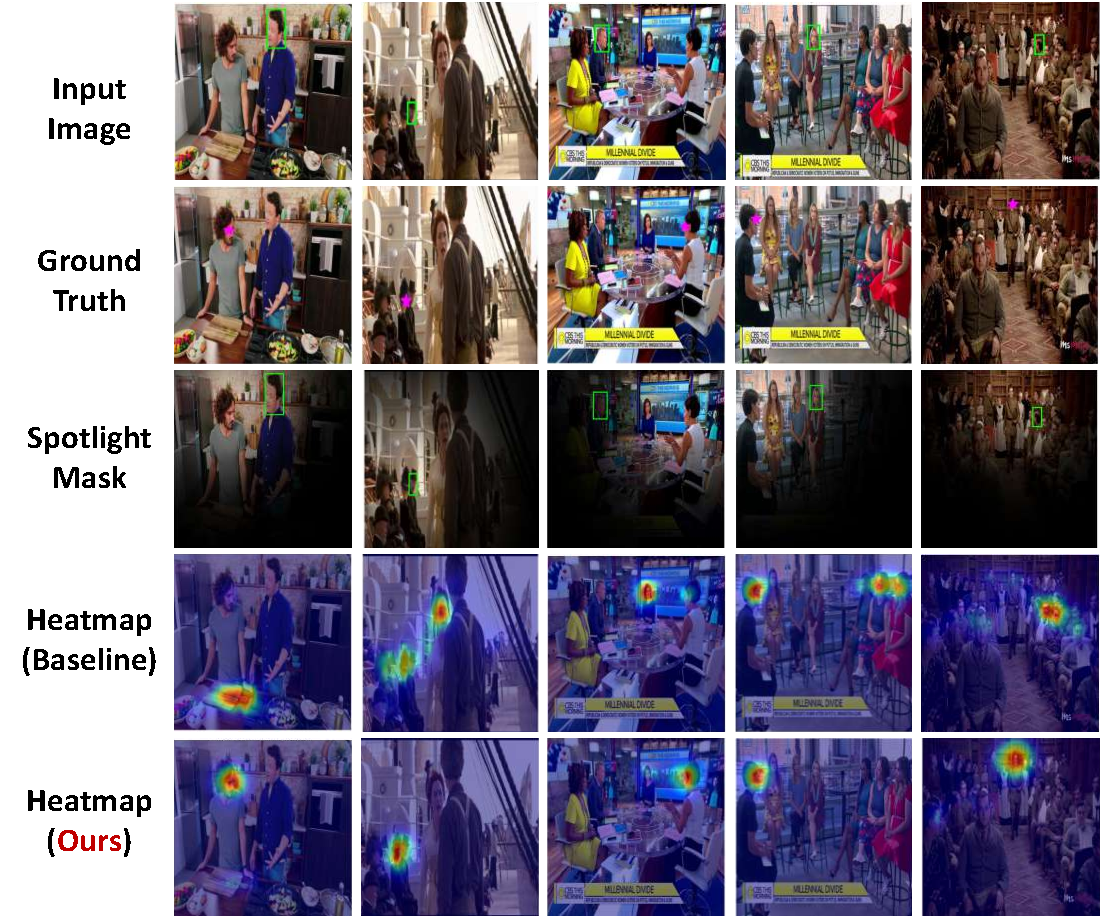
\includegraphics[width=\linewidth]{Figure/baseVSspot_compressed.pdf}
  \caption{Qualitative visual comparison between the baseline model and GazeSpot on the Crowd Subset. From top to bottom: input image with the target person's head annotated by a green bounding box, ground-truth fixation point annotation, frustum physical isolation mask generated by GazeSpot (Spotlight Mask), gaze heatmap predicted by the baseline model, and gaze heatmap predicted by our GazeSpot.}
  \label{fig:crowd_visualization}
\end{figure}
\textbf{Qualitative Evaluation}. To intuitively demonstrate the advantages in anti-interference capability, \autoref{fig:crowd_visualization} provides a qualitative visual comparison between the baseline model and GazeSpot on the Crowd Subset. Clearly, in complex scenes with dense crowd interference, the baseline model's attention is highly prone to diffusion. It is easily distracted by irrelevant background individuals possessing strong semantics, causing the predicted heatmap to deviate from the ground-truth fixation point. Conversely, relying on explicit geometric gating, GazeSpot effectively filters out background noise outside the viewing frustum, as illustrated by the Spotlight Mask in the figure. Even when facing interference from crowd occlusions, it still achieves highly compact and physically aligned spatial focus. This intuitively confirms the effectiveness of our proposed method in alleviating contextual interference.

\textbf{Model Complexity and Efficiency}.
While achieving exceptional robustness, GazeSpot maintains ultimate lightweight efficiency. Traditional multi-branch models easily incur parameter counts up to 50M or even over 100M. In contrast, since we completely freeze the foundation model, our GazeSpot possesses a mere 3.5M learnable parameters. As shown in \autoref{tab:sota_comparison}, compared to the baseline model Gazelle (2.8M), we only introduce a minuscule parameter overhead of 0.7M , primarily originating from the extremely lightweight SASA routing network and the GGSF gating MLP. This compellingly proves that the massive performance leap of GazeSpot in Crowd scenes stems from a profound physical mechanism reconstruction, rather than brute-force parameter stacking.

% [Placeholder for Table 4: Comparison of Model Complexity]
% \begin{table}[htbp]
%   \centering
%   \caption{Comparison of Param and FLOPs across different architectures. }
%   \label{tab:complexity}
%   \begin{tabular}{lcc}
%     \toprule
%     \textbf{Methods} & \textbf{Param (M)} $\downarrow$ & \textbf{FLOPs (G)} $\downarrow$ \\
%     \midrule
%     Fang et al.~\cite{fang2021dual} & 00.0 & 00.0 \\
%     Bao et al.~\cite{bao2022escnet} & 00.0 & 00.0 \\
%     Tafasca et al.~\cite{tafasca2023childplay} & 00.0 & 00.0 \\
%     ViTGaze~\cite{song2024vitgaze} & 00.0 & 00.0 \\
%     Gaze-LLE (ViT-B)~\cite{ryan2025gaze} & 2.8 & 00.0 \\
%     \midrule
%     \textbf{GazeSpot (ViT-B)} & \textbf{3.2} & \textbf{00.0} \\
%     \textbf{GazeSpot (ViT-L)} & \textbf{00.0} & \textbf{00.0} \\
%     \bottomrule
%   \end{tabular}
% \end{table}

\subsection{Ablation Study}
To validate the effectiveness of each core component, we conduct rigorous ablation studies on GazeFollow and VideoAttentionTarget. Results are presented in \autoref{tab:ablation}.

\textbf{Baseline (Last-layer only)}. Using only the deepest VFM features achieves 0.955 AUC and 0.107 $L_2$ error on GazeFollow. This validates our motivation: even with DINOv3's strong semantic capacity, single-layer representations hit a performance ceiling due to geometric detail loss.

\textbf{Effect of Multi-layer Fusion}. Simply concatenating multi-layer features without guidance (row 2) yields marginal and inconsistent gains, specifically \(+0.002\) AUC on GazeFollow and \(+0.004\) AUC on VideoAttentionTarget. We attribute this to low-frequency noise from shallow layers diluting the semantic signal because brute-force fusion lacks the adaptive routing required to resolve the spatial-semantic dilemma.

\textbf{Effect of SASA}. Adding the Scale-Aware Semantic Aggregation module (row 3) unlocks the potential of multi-layer features, improving GazeFollow AUC to 0.958 (+0.003 over raw concatenation) and reducing $L_2$ error to 0.102. The dynamic routing mechanism successfully extracts occlusion-resistant shallow edges when needed, as evidenced by the 9.0\% relative $L_2$ reduction (as shown in \autoref{tab:crowd_robustness}) in crowded scenes.

\textbf{Effect of GGSF}. Integrating the Geometry-Guided Spatial Focus atop SASA (row 4) constitutes the complete GazeSpot. This yields our final performance: 0.958 AUC and 0.101 $L_2$ on GazeFollow, 0.940 AUC and 0.099 $L_2$ on VideoAttentionTarget. The frustum isolation mechanism eliminates divergent activations behind the target, rendering heatmaps compact and physically aligned (\autoref{fig:crowd_visualization}).

\begin{table}[htbp]
  \centering
  \caption{Ablation study evaluating the individual contributions of Multi-layer Features, SASA, and GGSF on the GazeFollow and VideoAttentionTarget datasets (Backbone: DINOv3 ViT-B/16). The best results are highlighted in bold.}
  \label{tab:ablation}
  \resizebox{\linewidth}{!}{
  \begin{tabular}{ccccccc}
    \toprule
    \multirow{2}{*}{\textbf{Multi-layer}} & \multirow{2}{*}{\textbf{SASA}} & \multirow{2}{*}{\textbf{GGSF}} & \multicolumn{2}{c}{\textbf{GazeFollow}} & \multicolumn{2}{c}{\textbf{VideoAttentionTarget}} \\
    \cmidrule(lr){4-5} \cmidrule(lr){6-7}
    & & & \textbf{AUC} $\uparrow$ & \textbf{$L_2$} $\downarrow$ & \textbf{AUC} $\uparrow$ & \textbf{$L_2$} $\downarrow$ \\
    \midrule
    & & & 0.955 & 0.107 & 0.933 & 0.106 \\
    \checkmark & & & 0.957 & 0.103 & 0.937 & 0.103 \\
    \checkmark & \checkmark & & 0.958 & 0.102 & 0.939 & 0.101 \\
    \checkmark & \checkmark & \checkmark & \textbf{0.958} & \textbf{0.101} & \textbf{0.940} & \textbf{0.099} \\
    \bottomrule
  \end{tabular}
  }
% \vspace{-10pt}
\end{table}

\subsection{Analysis of Feature Over-smoothing}
\label{sec:experiments_45}
To deeply corroborate the hypothesis of ``feature over-smoothing in large models'' proposed in our \autoref{sec:introduction}, we conduct a feature-level analysis across different versions of DINO under the baseline architecture. The quantitative comparison is detailed in \autoref{tab:dino_oversmoothing}.

A counterintuitive phenomenon is observed: when utilizing a pure single-branch baseline architecture (extracting only the last-layer features), upgrading the backbone from DINOv2 to DINOv3 not only fails to bring performance improvements in gaze estimation but actually enlarges the $L_2$ error. The Principal Component Analysis (PCA) visualization (as shown in \autoref{fig:v2VSv3}) reveals its underlying pathology: DINOv3 possesses formidable global semantic homogeneity, yet exhibits severe feature over-smoothing in densely populated local regions. This over-smoothing erases the geometric boundaries between distinct individuals, causing the model to plunge into severe semantic confusion during prediction.

However, this phenomenon does not imply that DINOv3 is unsuitable. Precisely by leveraging the SASA routing and GGSF geometric gating mechanisms proposed by GazeSpot, we successfully leap over the resolution trap of DINOv3's last layer. By non-intrusively extracting its uncontaminated, early high-frequency features, we completely unleash the unfathomable representation potential of DINOv3. Experimental results show that DINOv3 equipped with the GazeSpot architecture achieves an overwhelming reversal, perfectly closing the loop on this paper's core argument regarding ``reconstructing the geometric-semantic balance'' of foundation models.

\section{Limitation}
Despite the effectiveness of the proposed approach, several limitations remain. The integration of multi-level feature aggregation inevitably introduces additional computational cost compared to lightweight single-layer designs such as Gaze-LLE, which may pose challenges for real-time deployment or resource-constrained scenarios.
In addition, the geometry-guided spatial constraint relies on the quality of head-related cues to construct the spatial prior. When head pose estimation becomes unreliable, particularly in cases of heavy occlusion or extreme viewpoints (as shown in \autoref{fig:limitation}), the resulting spatial constraint may be less accurate, potentially affecting overall performance.
% Another aspect worth noting is the generalization capability under highly unconstrained conditions. Although the model performs consistently on standard benchmarks, scenarios involving severe occlusion, unusual camera perspectives, or complex social interactions remain challenging, indicating that further improvements in robustness are still needed.
Future work may explore more efficient feature aggregation strategies, as well as adaptive spatial modeling mechanisms that can better handle uncertain or noisy geometric cues.

% [Placeholder for Table 6: Feature analysis table]
\begin{table}[htbp]
  \centering
  \caption{Performance comparison demonstrating the over-smoothing effect of DINOv3 in the baseline architecture, and the subsequent overwhelming reversal when integrated with the GazeSpot framework. All metrics report the $L_2$ error ($\downarrow$).}
  \label{tab:dino_oversmoothing}
  \resizebox{\linewidth}{!}{
  \begin{tabular}{lcccc}
    \toprule
    \multirow{2}{*}{\textbf{Dataset}} & \multicolumn{2}{c}{\textbf{Baseline (Gazelle)}} & \multicolumn{2}{c}{\textbf{GazeSpot (Ours)}} \\
    \cmidrule(lr){2-3} \cmidrule(lr){4-5}
    & \textbf{DINOv2} & \textbf{DINOv3} & \textbf{DINOv2} & \textbf{DINOv3} \\
    \midrule
    GazeFollow & 0.104 & 0.107 & \underline{0.102} & \textbf{0.101} \\
    VideoAttentionTarget & 0.107 & 0.106 & \underline{0.104} & \textbf{0.099} \\
    Crowd ($\geq 4$) & 0.133 & 0.139 & \underline{0.132} & \textbf{0.124} \\
    \bottomrule
  \end{tabular}
  }
\end{table}
\begin{figure}[htbp]
  \centering
  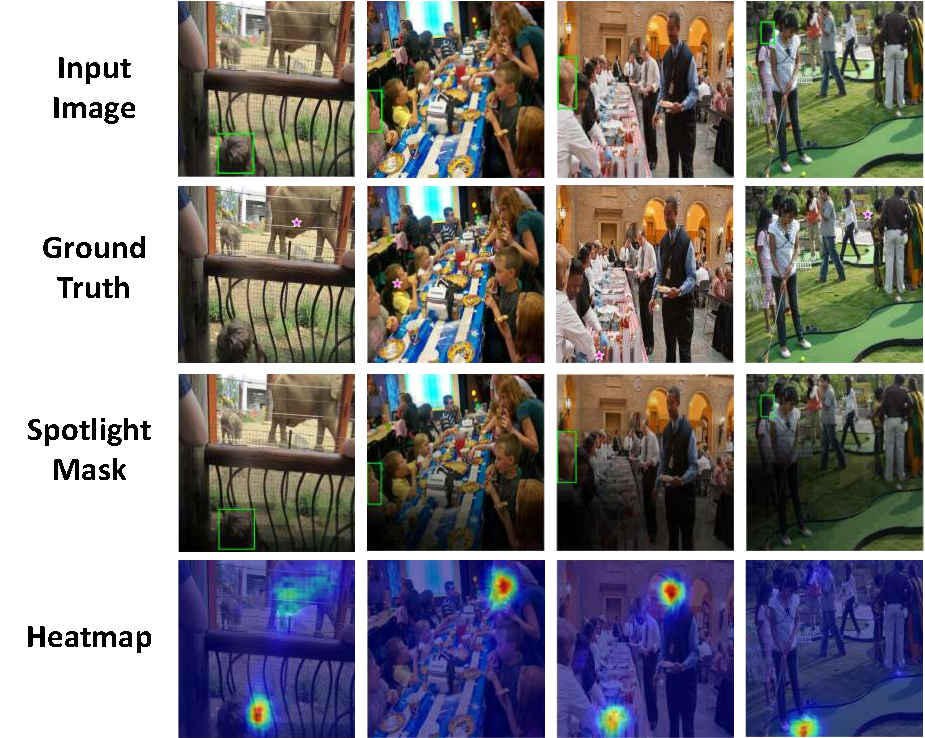
\includegraphics[width=\linewidth]{Figure/limitation_compressed.pdf}
  \caption{Visual examples of failure cases. In scenarios involving heavy head occlusion or extreme viewpoints, the spatial prior (Spotlight Mask) becomes unreliable, subsequently leading to inaccurate or diffuse gaze target predictions.}
  \label{fig:limitation}
\end{figure}
\section{Conclusion}
In this paper, we revisit gaze target estimation from the perspective of both representation and spatial reasoning. While recent approaches based on vision foundation models have achieved strong performance using simplified architectures, they largely rely on single-layer representations and implicit attention mechanisms, which may limit their effectiveness in complex scenes.
We show that accurate gaze estimation requires jointly modeling fine-grained spatial structures and high-level semantics. To this end, we propose a unified framework that integrates multi-level feature aggregation with geometry-guided spatial constraints. By leveraging complementary information across feature hierarchies and explicitly constraining the attention space, our approach improves robustness against contextual interference.
Extensive experiments on challenging benchmarks demonstrate that the proposed method consistently outperforms existing approaches, particularly in crowded scenarios.
Beyond gaze estimation, our findings suggest that combining multi-level representations with explicit spatial priors is a promising direction for improving dense prediction tasks based on vision foundation models.







%%
%% The acknowledgments section is defined using the "acks" environment
%% (and NOT an unnumbered section). This ensures the proper
%% identification of the section in the article metadata, and the
%% consistent spelling of the heading.
\begin{acks}
To Robert, for the bagels and explaining CMYK and color spaces.
\end{acks}

%%
%% The next two lines define the bibliography style to be used, and
%% the bibliography file.
\clearpage
\bibliographystyle{ACM-Reference-Format}
\bibliography{sample-base}


%%
%% If your work has an appendix, this is the place to put it.


\end{document}
\endinput
%%
%% End of file `sample-sigconf-authordraft.tex'.
